% https://tex.stackexchange.com/questions/749936
\documentclass[border=5pt]{standalone}
\usepackage{tkz-euclide}
\begin{document}
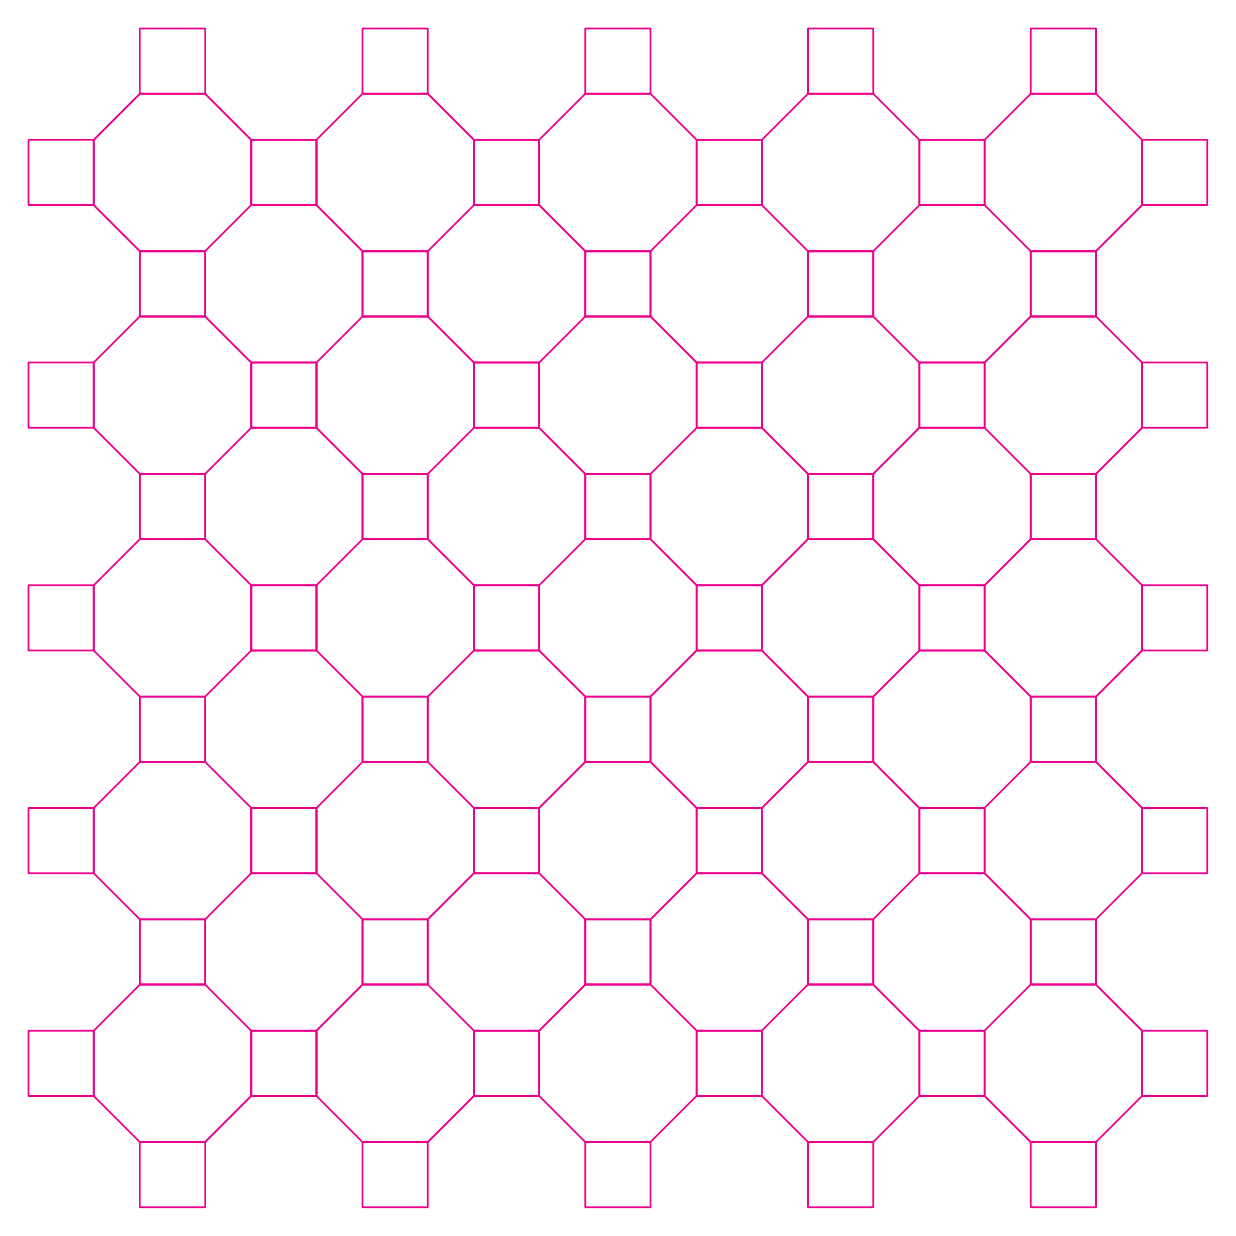
\begin{tikzpicture}[
    myunit/.pic={
        \tkzDefPoints{0/0/O,1/\tkzSqrTwo-1/x}%
        \tkzDefRegPolygon[center,sides=8,name=P](O,x)
        \tkzDrawPolygon[#1](P1,P...,P8)
        \tkzDefSquare(P3,P2)\tkzGetPoints{Q2}{Q3}
        \tkzDrawPolygon[#1](P2,P3,Q3,Q2)
        \tkzDefSquare(P1,P8)\tkzGetPoints{Q1}{Q8}
        \tkzDrawPolygon[#1](P1,P8,Q1,Q8)
        \tkzDefSquare(P7,P6)\tkzGetPoints{Q7}{Q6}
        \tkzDrawPolygon[#1](P6,P7,Q6,Q7)
        \tkzDefSquare(P5,P4)\tkzGetPoints{Q4}{Q5}
        \tkzDrawPolygon[#1](P4,P5,Q5,Q4)
    }
]
\foreach \x in {0,...,4}{
    \foreach \y in {0,...,4}{
        \pic at (\fpeval{2*\x*\tkzSqrTwo},\fpeval{2*\y*\tkzSqrTwo}) {myunit={magenta,semithick}};
    }
}
\end{tikzpicture}
\end{document}